\section{Server Design}

The server is the central component of \snowman{} and generally consists of:

\begin{itemize}
  \item Central rule storage
  \item Web interface for user interaction
  \item Update module to get updates from rule sources
  \item RPC interface to communicate with the clients 
\end{itemize}

The central storage of rules would be in a normal relational database. As we
have decided to use \django{} (described in Chapter \ref{chap:implementation})
as our framework, we have a great flexibility in selecting the database we actually
use. The current version of \django{} (1.6) supports MySQL,
PostgreSQL, SQLite and Oracle. For the RPC interface, we have decided to use
XML-RPC. This is a very simple protocol using XML over HTTP to transfer 
requests and data to and from the server. To be able to keep up with the aspect
of privacy and security, we encrypt the raw HTTP stream using SSL. 

\subsection{Architecture}

We have designed the server by the layered approach of MVC (figure
\ref{fig:server_architecture}).

\begin{figure}[h]
	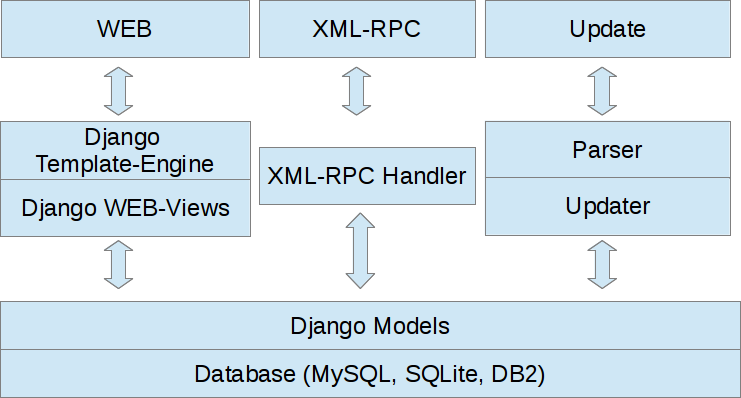
\includegraphics[width=130mm]{./img/Server-MVC.png}
	\caption{Server Architecture}
	\label{fig:server_architecture}
\end{figure}

The web-interface uses pure \django{} logic. The HTML visible in the users
browser is generated by the \django{} template-engine, which recieves its data
from the views created by using ordinary Python code.

The XML-RPC server uses a handler which is administering the connections to
and from the sensors, and exposing the relevant methods to allow the sensors to
do a synchronization.

The update module is used for unpacking and preparing the update files for
parsing. It then handles the files to the parser. This parser is then tasked
with translating the raw rule files into more managable datastructures for the
Updater, which in turn saves them to the database.

Finally, common for all the interfaces is the \django{} Models. We use the
database abstraction layer provided by \django{} to map the rows of a
relational database into \django{} objects. This is the part that lets us write
code which is compatable with several different database engines.

\subsection{User interface}
The main user-interface for snowman is the web-interface. It is based on
django's template-system for the generation of html which is displayed in the
web-browser on the user's computer.

The web-interface uses javascript to dynamicly be able to load/change the
content of the pages without refreshing the whole page. Important parts of the
webinterface is possible to download using AJAX, to update tables and simmilar.

Javascript is also used to improve the user-experience of the interface, due to
functionality which a moden computer-user expects from modern web-pages.

\subsubsection{Url's}

The first step of serving a page to a user is a HTTP request for a specific page
is recieved. The pages are uniqely identified by url's, like '/web/rules/'.

The url's are structured in a logical manner, where everything in the
webinterface is found under /web/, everything regarding the administration of
rules is found under /web/rules/, etc. The url's might contain dynamic data,
like pagenumbers (ie: /web/rules/rules/page/3/ which will give you the third
page of the rule-list), so that dynamic content can be loaded dynamicly when
needed.

Django uses the urls to identify which views the requested url corresponds to.
When a view is identified, the request (and its dynamic content) is passed to
the corresponding view.

\subsubsection{Views}

The views is the part of the user-interface which collects the required data
from the models-layer, and generates a response to the web client. The response
can contain a full web-page, or just a small subset of one if the request was
issued by AJAX.

The typical steps a view makes, to generate a response would be:
\begin{enumerate}
  \item Collect the requiered data from the database(s) using the \django{}
  models.
  \item Hand the collected data, and a template, to the template-engine to
  generate the HTML representing the webpage the user want.
  \item Send the created webpage as a response to the user.
\end{enumerate}

The view-system decides what to show, and then lets the template-system decide
how to show it. The view-system in itself is not creating any html or simmilar.
It soley creates data-structures.

If the request was for some data, and not a webpage, step 2 in the list above
might be skipped, and instead return the data as JSON or simmilar in step 3.

If errors oocures in the view-system, appropriate exception can be raised to
tell \django{} to return an error-code or an error-page to the user, instead of
what the user requested.

\subsubsection{Templates}

When the view-system have prepared all the data, the template-system takes over.
The job of the templates is to take the supplied data, and inject it into
pre-made skeletons of HTML. This way, all the design/display part of the
webinterface is collected to one single place, and that give us a very clear
line between data and design.


\subsection{Database}

As the database of the server is quite complex, we have divided the drawings, so
that we have one drawing per module.

\subsubsection{Core}

The core database-architecture used for storing the rules is described in
figure \ref{fig:server_database_core}. 

\begin{figure}[h]
        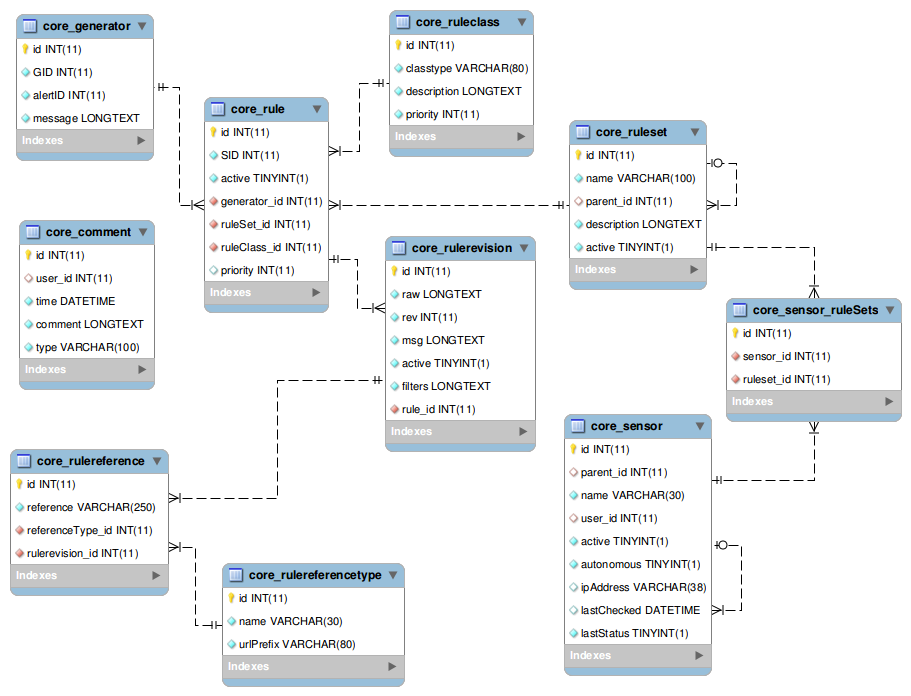
\includegraphics[width=127mm]{./img/Server-DB-Core.png}
        \caption{Core server-database}
        \label{fig:server_database_core}
\end{figure}

The most central part of our system is the representation of a Rule. A single
Rule might have several Revisions, as we might want to keep some history when
they get updated. Each Revision have its own set of References attached.

A single Rule also have a lot of other properties which it might share with
other Rules. A Generator, a Classification and a Ruleset are examples of such.

Finally, the Rules are assigned to a Sensor by attaching Rulesets to the
Sensor.

\subsubsection{Tuning}

In addition to storing the raw rules, we would like to be able to store
tuning parameters on the rules. As sensors might have different
tuning parameters, we cannot attach the tuning directly to the rules. Separate
tables (as described in figure \ref{fig:server_database_tuning}) is thus needed
to model the tuning parameters.

\begin{figure}[h]
        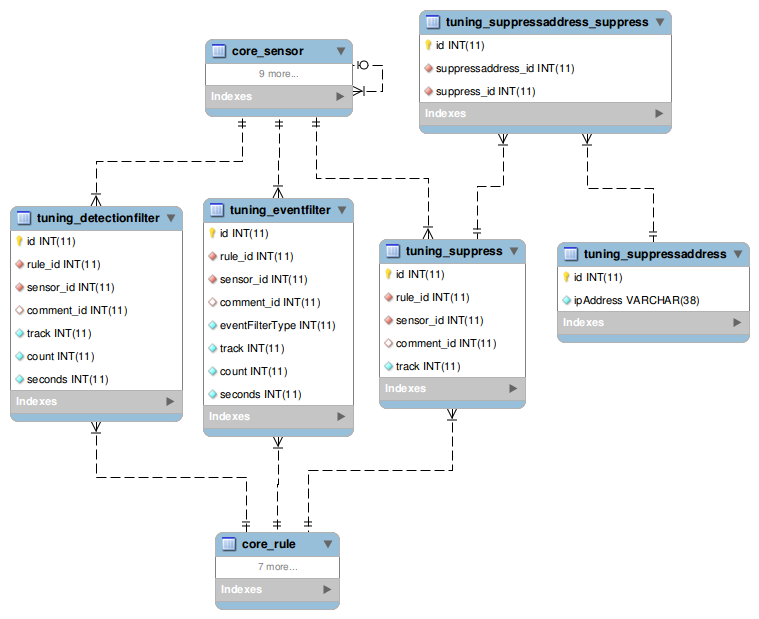
\includegraphics[width=127mm]{./img/Server-DB-Tuning.png}
        \caption{Tuning server-database}
        \label{fig:server_database_tuning}
\end{figure}

Both types of filters, and the suppressions are connected to a Rule and a
Sensor. This way, we let the user spesify filters for the individual sensors.
If a sensor does not have a filter applied, but any parent sensor of that sensor
has one, the closest parent's filter will be applied.

\subsubsection{Update}

When rules are inserted to the database, we would like to have some traceability
to be able to determine where and when a rule has entered our system. To be
able to do this, we have the update object (figure
\ref{fig:server_database_update}).

\begin{figure}[h]
        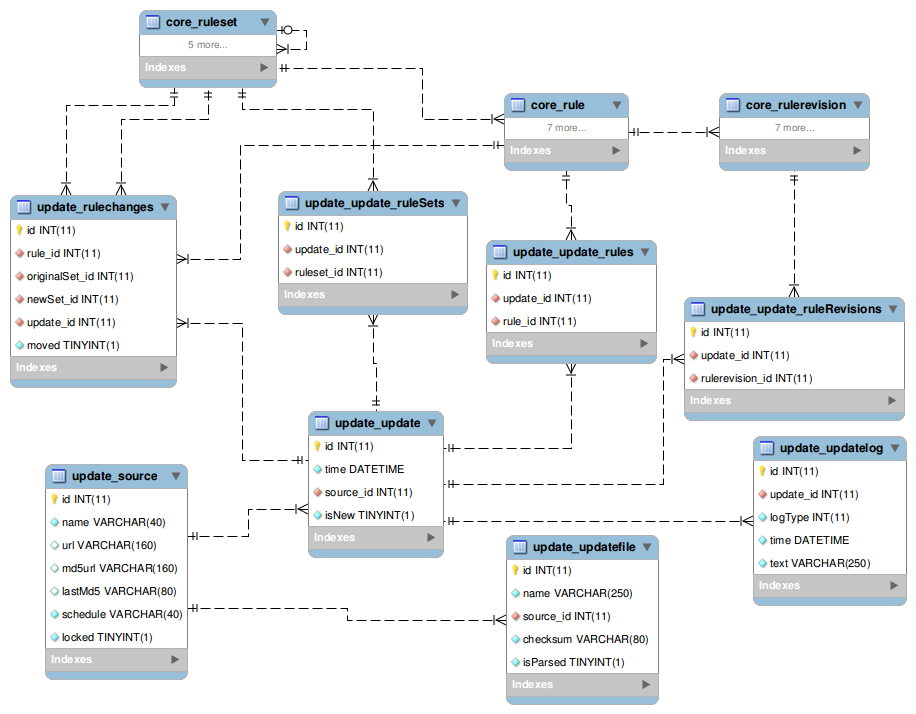
\includegraphics[width=127mm]{./img/Server-DB-Update.png}
        \caption{Update server-database}
        \label{fig:server_database_update}
\end{figure}

The structure of update lets us store the update sources,
and add an update object for each update ran from a given source. These update
objects can in turn have relations to rules, rulesets and rulerevisions, so
that we can track changes for each update.
